%Functionality to process and replay execution logs is key to the success of our approach.
%However unlike the example applications described
%by the delta debugging paper~\cite{Zeller:1999:YMP:318773.318946}, the system we are troubleshooting is not a
%single program---it encompasses all the nodes and links of a distributed system,
%including controllers, switches, and end-hosts, where asynchrony
%makes it difficult to reliably replay inputs.

Our technique depends on infrastructure for testing SDN control software.
All three of the major commercial SDN controller teams that we have first-hand knowledge of employ a team of QA
engineers to fuzz test their controller software on testbeds of switches and hosts.
As depicted in Figure~\ref{fig:qa_cluster},
this fuzz testing infrastructure
consists of the controller software under test, the network testbed (which may
be software or hardware), and a centralized
test orchestrator
that chooses random input sequences, drives the behavior of the testbed,
periodically checks invariants, and manages log files. When a bug is discovered, an
engineer triages it and then sends logs to a developer for further troubleshooting.

\begin{figure}[tb]
    \hspace{-10pt}
    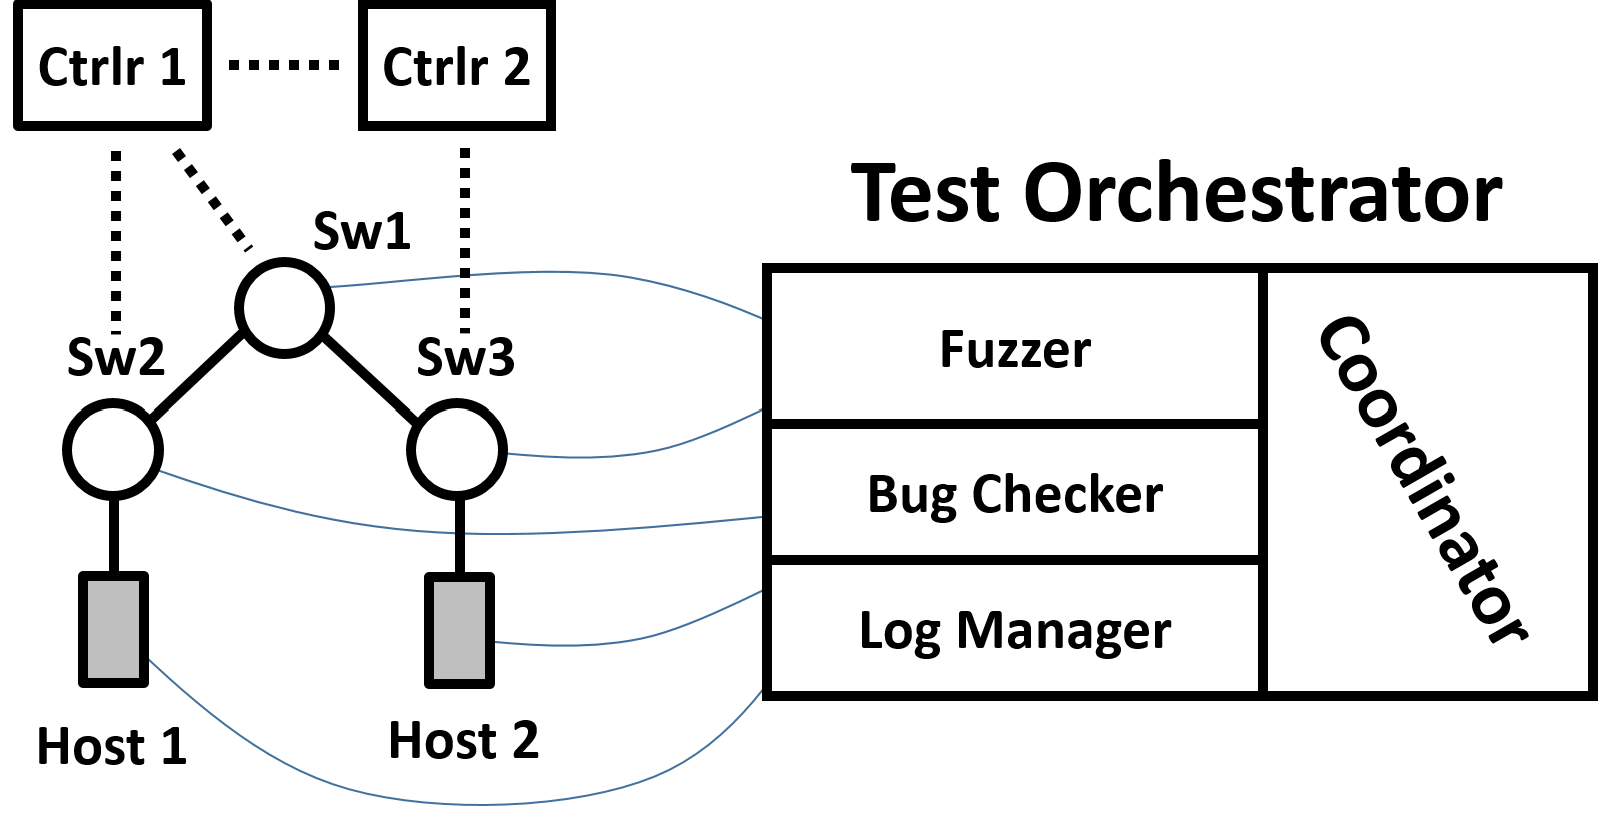
\includegraphics[width=3.25in]{../diagrams/architecture/qa_cluster.pdf}
    \caption[]{\label{fig:qa_cluster} Typical QA testbed. A centralized test
    orchestrator injects inputs and checks invariants}
    \vspace{-1em}
\end{figure}

Engineering organizations with existing
QA testbeds can add delta debugging to their test
orchestrator, and optionally add interposition points throughout the
testbed to control event ordering during replay.
In this way they can continue simulating large scale networks with
the switches, middleboxes, hosts, and routing protocols they had already
chosen to include in their QA testbed.

We do not have access to such a QA testbed, and instead built our own
testing framework to discover bugs and
perform replay. Our framework mocks out the control plane
behavior of network devices in lightweight software switches and hosts (with
support for minimal data plane forwarding).
We then run the control software on
top of this \tester~and connect the software switches to the
controllers. This design is similar to production software QA testbeds. % as if they were true network devices
%, such that the controllers believe they are configuring a true %network.
Our \tester~also implements delta debugging and interposes and buffers messages on all communication
channels, allowing it to delay, drop, or reorder
messages as needed to induce failure modes during testing. This interposition
allows us to replicate many of the failure modes caused by asynchrony in real
networks in a more deterministic manner. During
replay, we use these buffers to enforce event orderings by
matching messages in the buffers by their fingerprints and managing
the order in which messages are let through. The overall architecture is depicted in
Figure~\ref{fig:architecture}.

\begin{figure}[tb]
    %\hspace{-10pt}
    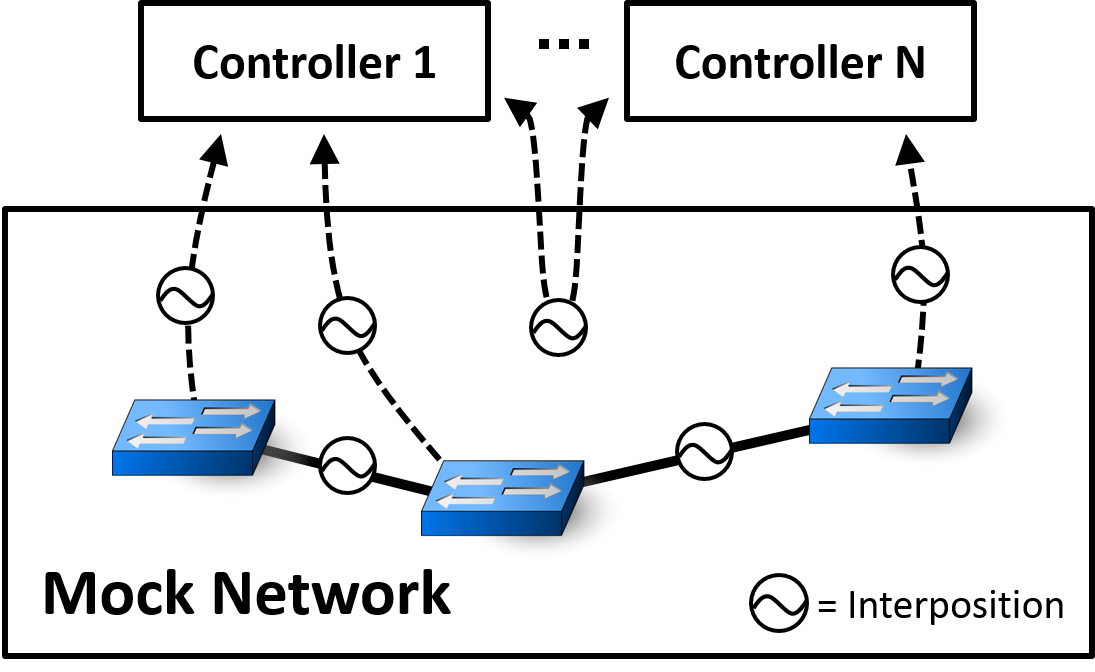
\includegraphics[width=3.25in]{../diagrams/architecture/Debugger_Architecture.png}
    \caption[]{\label{fig:architecture} \projectname~runs mock
    network devices, and interposes on all communication
    channels.}
    \vspace{-1em}
\end{figure}

% \begin{table}
% \centering
% \begin{tabular}{|ll|}
% \hline
% - All-to-all reachability & - Loop freeness \\
% - Blackhole freeness & - Controller liveness \\
% - POX ACL compliance & - ONOS flow routing compliance \\
% \hline
% \end{tabular}
% \caption{Invariant checks currently supported by \projectname}
% \label{tab:invariants}
% \end{table}

We begin by using our \tester~to perform testing on controllers to find
bugs. Most commonly we generate randomly chosen input
sequences~\cite{Miller:1990:ESR:96267.96279}, feed them to controller(s),
and monitor
invariants at chosen intervals.\footnote{We currently support the following invariants:
  (a) all-to-all reachability, (b) loop freeness, (c) blackhole freeness, (d) controller
liveness, and (e) POX ACL compliance.
  %The full list of invariants currently supported is shown in Table~\ref{tab:invariants}
}
We also run the \tester~interactively
so that we can examine the state of any part of the network,
observe and manipulate messages, and follow our
intuition to induce orderings that we believe may trigger bugs.
Either way, controlling the inputs from a single location
allows our test framework to record a global, serial
event ordering.

After discovering an invariant violation of interest, our system replays
the logged sequence of inputs (shown in Table~\ref{tab:inputs}). For example,
the system replays link failures
by disconnecting the edge in the \tester, and sending an
\verb=ofp_port_status=~\cite{openflow} message from the adjacent switches to their parent controller(s).

\projectname~is our realization of this system and is implemented in more than 21,000 lines of Python in
addition to the Hassel network invariant checking library~\cite{hsa}.
\projectname~also optionally makes use of Open vSwitch~\cite{pfaff2009extending} as an interposition point for
messages sent between distributed controllers. We have
made the code
for \projectname~publicly available at \href{http://ucb-sts.github.com/sts}{ucb-sts.github.com/sts}.
% and have discussed the logistics of deploying it with several SDN companies.

\colin{TODO: Discuss the value of replay for root causing here? Or just let
the use cases speak for themselves?}
%How do we ensure the same scheduling order of controller processes? (see
%Section 4.5 of ReVirt\cite{Dunlap:2002:REI:844128.844148}). We observe that the controllers do not use any shared
%memory communication.}

\subsection{Coping with Non-Determinism}
\label{subsec:coping}

Non-determinism in the execution of concurrent processes stems from
differences in system call return values, process scheduling decisions (which can
even affect the result of individual instructions, such as x86's
interruptible block memory instructions~\cite{Dunlap:2002:REI:844128.844148}),
and asynchronous signal
delivery. These sources of non-determinism can affect whether \projectname~is
able to reproduce the original bug during replay.

Most testing systems, such as the QA testing frameworks we are
trying to improve, do not attempt to mitigate non-determinism.
%;they assume
%that developers will be able replicate bugs by attempting to reproduce the
%same conditions as the original test run, else track down the root cause
%only by
%inspecting the raw execution logs.
\projectname's main approach to coping with non-determinism
is to replay each subsequence chosen
by delta debugging multiple times. If the non-deterministic bug occurs with
probability $p$, we can model the probability that we will observe it within $r$ replays as $1-(1-p)^{r}$. This exponential
works strongly in our favor; for example, even if the original bug is
triggered in only 20\% of replays, the probability that we will not trigger
it during an intermediate replay is approximately
1\% if we replay 20 times per subsequence.\footnote{See
\S\ref{subsec:multiple_replays} for an experimential evaluation of this model.}
\colin{Mention optimizing for reproducibility?}

\subsection{Mitigating Non-Determinism}
\label{subsec:mitigating}

When non-determinism acutely impacts replay, one might also seek to mitigate or prevent non-determinism altogether.
Deterministic replay techniques~\cite{Dunlap:2002:REI:844128.844148,Geels:2006:RDD:1267359.1267386},
which precisely record and replay system call return values and process
scheduling decisions,
may be deployed to reliably produce bugs in exchange for a loss in performance.
Unfortunately these techniques do not easily allow any modifications to the inputs fed to the
processes during replay, since changes may cause the remaining execution to
subtly differ (\eg~the sequence numbers of packets may all differ), and our
%This precludes the possibility of employing (fully) deterministic replay techniques in
%\projectname,
goal is precisely to modify (eliminate) the inputs fed to the
distributed system.
%And even if these sources were
%eliminated, it would not be possible to achieve perfectly deterministic
%replay in all cases without full visibility into internal events--a daunting
%instrumentation task.

We therefore strived to balance resilience to non-determinism and the need
to modify control software. We placed \projectname~in a position to
record and replay all network events in serial order, and ensured that all
data structures within \projectname~were unaffected by randomness. For example,
we avoid using hashmaps that hash keys according to their memory address,
and sort all list return values.

We also optionally interpose on the controller software itself.
Routing the {\tt gettimeofday()} syscall through \projectname~helps ensure timer
accuracy.\footnote{When the pruned trace differs from the original, we make a
best-effort guess at what the return values of these calls should be. For example,
if the altered execution invokes {\tt gettimeofday()} more times than we recorded
in the initial run, we interpolate the timestamps of neighboring events.}\footnote{Only
supported for POX and Floodlight at the moment.} When sending data over multiple sockets, the operating system exhibits
non-determinism in the order it schedules I/O operations.
\projectname~optionally ensures a deterministic order of messages
by multiplexing all sockets
onto a single true socket. On the controller side \projectname~currently
adds a shim layer atop the control
software's socket library,\footnote{Only supported for POX at the moment.} although this
could be achieved transparently with a libc shim layer~\cite{Geels:2006:RDD:1267359.1267386}.
%In the future we plan to implement deterministic message ordering without code modifications by
%loading a shim layer on top of
%libc (similar to liblog~\cite{Geels:2006:RDD:1267359.1267386}).

\projectname~may need visibility into the control software's internal state
transitions to properly maintain happens-before relations during replay. We
gain visibility by making a
small change to the control software's logging library\footnote{Only supported
for POX and Floodlight at the moment.}: whenever a control process executes a log
statement, which often indicates that an important state transition is about to take
place, we notify \projectname. Such coarse-grained visibility into internal
state transitions does not handle all cases, but we find it suffices in practice.\footnote{We discuss this limitation further in \S\ref{subsec:non_goals}.}
We can also optionally use
logging interposition as a
synchronization barrier, by blocking the process when it executes crucial logging statements
until \projectname~explicitly tells the process that it may proceed.

%If blocking was enabled
%during recording, we force the control software to block at internal state
%transition points again during replay
%until \projectname~gives explicit acknowledgment.

\subsection{Checkpointing}
\label{subsec:snapshotting}

To efficiently implement the {\sc Peek()} algorithm depicted in
Figure~\ref{fig:peek} we assume the ability to record checkpoints of the state of the
system under test. We currently implement checkpointing for the POX
controller\footnote{We only use the event scheduling heuristics described in
\S\ref{subsec:timing_heuristics} for the other controllers.} by telling it to \verb=fork()= itself and suspend its child,
cloning the sockets of the parent
(which constitute shared state between the parent and child processes,
since the socket state is managed by the kernel),
and later resuming the child. This simple mechanism does
not work for controllers that use other shared state such as disk.
To handle other shared state one could checkpoint processes within
lightweight Unix containers~\cite{lxc}. For distributed controllers, one
would also need to implement a consistent cut
algorithm~\cite{Chandy:1985:DSD:214451.214456}, which is available in several open source
implementations~\cite{ansel2009dmtcp}.

If developers do not choose to employ checkpointing,
they can use our implementation of {\sc Peek()} that replays the prefix for each input
interval from the beginning of the trace, thereby increasing replay runtime by
a factor of $n$. Alternatively, they can
avoid {\sc Peek()} and solely use the event scheduling heuristics described in \S\ref{subsec:timing_heuristics}.

Beyond its use in {\sc Peek()}, snapshotting has three advantages.
As mentioned in \S\ref{subsec:complexity}, only considering events starting
from a recent checkpoint rather than the beginning of the execution decreases the number of events to
be minimized. By shortening the replay time, checkpointing coincidentally helps cope
with the effects of non-determinism, as there is less opportunity for
divergence in timing. Lastly, checkpointing can improve the runtime of delta
debugging, since many of the subsequences chosen throughout delta debugging's
execution share common input prefixes.

\subsection{Timing Heuristics}
\label{subsec:timing_heuristics}
\colin{TODO: add more experiments here}

We have found a number of
heuristics useful for ensuring that invariant violations are consistently reproduced during replay.
These heuristics may be used alongside or instead of {\sc Peek()}. We evaluated the effectiveness
of these heuristics using visualization tools
(described in \S\ref{subsec:root_causing}) to compare replay executions with and
without the heuristics enabled.

\noindent{\bf Event Scheduling.} If we had perfect visibility into
the internal state transitions of control software, we would be able to replay inputs at precisely the correct point in
the happens-before relation. Unfortunately this is impractical.

We find that keeping the wall-clock spacing between replay events
close to the recorded timing helps (but does not alone suffice) to
ensure that invariant violations are consistently
reproduced. When replaying events, we \verb=sleep()= between each
event for the same duration that was recorded in the original trace,
less the time it takes to replay each event. Accounting for the
extra time it takes to replay events is especially important when we
time out on internal events, or when input events take a long time to inject.

\noindent{\bf Whitelisting keepalive messages.} We observed during some
of our experiments that the control software incorrectly inferred that links or switches had
failed during replay, when it had not done so in the original execution.
Upon further examination we found in these cases that LLDP and OpenFlow echo
packets periodically sent by the control software were
staying in \projectname's buffers too long during replay, such that the
control software would time out on them. To avoid these differences in timing
we added an option to always pass through
keepalive messages that mitigates the issue. The limitation of this
heuristic is that it cannot be used on bugs involving keepalive messages.

%We also tried another algorithm: let new
%internal messages through, keep a window of what we expect. If we don't
%expect, let it through. Problem: false positive: accidentally let through
%internal messages too early, then we time out on them after.

\noindent{\bf Whitelisting dataplane events.} Dataplane forward/drop events constitute a
substantial portion of overall events. However, for
many of the controller applications we are interested in, dataplane
forwarding is only relevant insofar as it triggers control plane events
(\eg~host discovery). We find that allowing dataplane forward events through by
default, \ie~never timing out on them during replay, can greatly decrease
skew between the wall-clock timing of the original vs.\ replayed trace.
%we keep a window of expected
%dp *drops* into the future. We then allow the dp packet through, *unless* we
%see that we should drop it in the near future.

% \noindent{\bf Using logging statements as barriers.} We briefly experimented
% with using logging statements within control software to manipulate its execution speed,
% for use in the rare cases in which we observed high variability in the
% controllers' response time. Our technique is to cause our logging
% interposition layer to block the entire controller
% process each time it issues a logging statement until \projectname~gives it
% explicit permission to proceed. We found that some care is needed to deal
% with unexpected state transitions, since the controller process will block
% indefinitely until \projectname~gives it acknowledgment.
% We currently turn this heuristic off by default.

\subsection{Root Causing Tools}
\label{subsec:root_causing}

Throughout our experimentation with \projectname, we often found that
minimized event traces alone were insufficient to
pinpoint the root causes of bugs. We therefore implemented a number of
complementary root
causing tools within \projectname,
which we use along with Unix utilities to help us complete the final
stage of debugging. We illustrate in \S\ref{sec:evaluation}~how exactly we use
these tools.

\noindent{\bf OFRewind}. \projectname~supports an interactive replay mode
similar to OFRewind~\cite{ofrewind} that allows troubleshooters to query the
state of the network throughout replay, filter subsets of the events, check
additional invariants, and
even induce new events that were not part of the original event trace.
\colin{Cut if we need space:} Similar to OFRewind, we do not run concurrent controller processes while the
user is interactively performing replay, since proper replay across
concurrent processes requires precise timing.
Instead, \projectname~replays the exact OpenFlow commands from the
original trace to the switches, and creates mock TCP connections that drop
whatever messages the switches attempt to send back to the controllers.

\noindent{\bf Packet Tracing}. Especially for SDN controllers that react to
flow events, we found it useful to trace the path of individual
packets throughout the network. \projectname~includes tracing instrumentation
similar to NetSight~\cite{ndb14} for this purpose.

\noindent{\bf OpenFlow Reduction}. The OpenFlow commands sent by controller software
are often somewhat redundant. For example, controllers may override routing
entries, allow them to expire, or periodically flush the
contents of flow tables and later repopulate them. \projectname~includes a
tool for filtering out such redundant messages,
leaving only those commands that are directly relevant for invalid network
configurations.

\noindent{\bf Event Visualization}. Understanding the timing of messages and internal
state transitions is a crucial part of troubleshooting distributed systems.
STS includes two visualization tools designed to aid with this task. First, we
include a tool to visualize space-time diagrams~\cite{Lamport:1978:TCO:359545.359563}
of event traces.
%, such as the one depicted in Figure~\ref{fig:example}.
Second, we include a tool to visually highlight event ordering differences
between two or more event traces, which is especially useful for comparing the behavior of
intermediate delta debugging replays when the original trace exhibits a high degree of non-determinism.

\eat{
\subsection{Scaling and Parallelization}
When minimizing very large event traces we found that the garbage collector
for our \tester~often became overwhelmed (causing the process to slow down
substantially) after replaying several subsequences, since each replay could
occupy gigabytes of memory with many small objects.
After observing this behavior, we modified \projectname~to fork a process
(either local or remote) for each subsequence chosen by delta debugging,
and gather the results of the replay via RPC; the OS cleans up the forked process,
eliminating garbage collection overhead.
As an added benefit, this architectural change allows us to support
parallelized delta debugging across multiple cores or machines.
}

\subsection{Limitations}
\label{subsec:non_goals}

Having detailed the specifics of our approach we now
clarify the scope of our technique's use.

\noindent{\bf Partial Visibility.} Our event scheduling algorithm assumes that
it has visibility into the occurrence of relevant internal events. For
some controllers this may involve substantial instrumentation effort beyond
pre-existing log statements, though as we show in our evaluation, most bugs
we encountered can be minimized without perfect visibility.

\noindent{\bf Non-determinism.} Non-determinism
is fundamental in networks. When non-determinism is present
\projectname~(i) replays multiple times per subsequence, and (ii) employs
software techniques for mitigating non-determinism, but it may nonetheless
output a non-minimal causal sequence. In the common case this is still
better than what developers had before, since developers generally
do not have tools for reproducing non-deterministic bugs.
In the worst case \projectname~leaves the
developer where they started: an unpruned log.

%In particular our technique is not designed to reproduce bugs
%involving non-determinism within a single controller (\eg~race-conditions between threads);
%we focus on coarser granularity errors (\eg~incorrect failover logic).

\eat{
\noindent{\bf Troubleshooting vs.\ Debugging.} Our technique is a troubleshooting tool, not a debugger;
by this we mean that our approach helps identify and localize inputs that
trigger erroneous behavior, but it does not directly identify which
line(s) of code cause the error.
}

\noindent{\bf Bugs Outside the Control Software.} Our goal is not to find the root
cause of individual component failures in the system (\eg~misbehaving routers,
link failures). Instead, we focus on
how the distributed system as a whole reacts to the occurrence of such inputs.
%If there is a bug in your switch, you will need to contact your hardware vendor;
%if you have a bug in your policy specification, you will need to take a closer look at what you specified.

\eat{
\noindent{\bf Globally vs.\ Locally Minimal Input Sequences.}
Our approach is not guaranteed to find the globally minimal
causal sequence from an input trace, since this involves enumerating the powerset of
$E_L$ (a $O(2^n)$ operation).
The delta debugging algorithm we employ does provably find a
locally minimal causal sequence~\cite{Zeller:1999:YMP:318773.318946},
meaning that if any input from the sequence is pruned, no invariant violation
occurs.
}

\noindent{\bf Correctness vs.\ Performance.}
We are primarily focused on correctness bugs, not performance bugs.

\eat{
\noindent{\bf Bugs Found Through Fuzzing.}
We generate bugs primarily through fuzz testing, not by finding them in
operational traces. There is a substantial practical hurdle in instrumenting
operational systems to produce logs that can be injected into our system, as
discussed in \S\ref{subsec:production_logs}.
}
% , and we have not addressed those issues yet.
%In practice some bugs
%found through fuzzing will not be considered worthwhile to investigate.

\eat{
\noindent{\bf Scaling.}
Our discussions with companies with large SDN deployments suggest that scaling to the size of the
large logs they collect will be a substantial challenge.
On the other hand, the fact that these logs are so large makes the need for finding MCSes even more acute.
}

\eat{
\noindent{\bf Proactive vs.\ Reactive Configuration.} We focus primarily on
\emph{proactive} configuration, where controllers react to policy and topology changes, but
not necessarily individual packets or flows events in the
dataplane.\footnote{Production controllers typically adopt this model for
performance reasons.}
The main challenge in extending our approach to reactive controllers is
achieving efficient simulation of dataplane traffic.
\andi{Could cut this. We actually find reactive bugs}
}

